
The participating roles in the software development process are defined in
CENELEC EN 50128 Figure~2 (see Figure~\ref{fig:preferred-roles}. In the
following all references to ``the standard'' will refer to CENELEC EN
50128:2011~\cite{EN-50128}.

We will first list and describe the roles in
Section~\ref{sec:participating-roles}, then we will shortly describe the SW
planing phase in Section~\ref{sec:documents--plan} and present the overall
lifecycle phases in Section~\ref{sec:lifecycle-phases}. A detailed description
for the system development phase is given in Section~\ref{sec:syst-devel-phase}
and for each of the SW development phases in
Section~\ref{sec:sw-development-phase}. Section~\ref{sec:conclusion-fm-process}
gives a short conclusion on the proposed development process for openETCS.

\subsection{Participating Roles}
\label{sec:participating-roles}

Each of the participants must be noted and her name and role recorded. Which
role can be taken by the same person is regulated as shown in
Figure~\ref{fig:preferred-roles}.

\subsubsection{Requirements Manager (RQM)}
\label{sec:requ-magang-rqm}

The main task of the RQM is to take care of the software requirements. She will
specify the software requirements, ensure their traceability wrt. system level
requirements and ensure the consistency of the SW requirement specification.

\subsubsection{Designer (DES)}
\label{sec:designer}

The main task of the DES is to create acceptable solutions from the SW
requirement specifications. She is responsible for the decisions which design
methods to apply and which tools to use. The DES develops the software component
specifications and ensures their traceability and consistency wrt. SW
requirements specification.

\subsubsection{Implementer (IMP)}
\label{sec:implementer}

The main task of the IMP is the transformation of the software design solution
into source code, DSLs or other appropriate formalisms. Besides the
implementation she will produce the documentation describing the implementation,
the applied methods, data types and data structures. She will also ensure the
traceability wrt. SW design. The IMP will apply the specified coding standards,
use the specified programming languages and use safety design principles.

\subsubsection{Tester (TST)}
\label{sec:tester}

The TST is responsible for the planning of all test activities and will produce
the test specification which includes the test cases and their objectives. She
is responsible to assure the execution of the SW tests, the recording of their
outcomes and to select the test equipments and methods. The TST will communicate
relevant deviations from the specifications to the change management.

\subsubsection{Verifier (VER)}
\label{sec:verifier}

The VER is responsible to produce the SW verification plan which specifies what
and how it has to be verified and what has to be produced as evidence. She will
evaluate all deviations from the verification plan according to their potential
impact and risk and communicate all deviations to the change management. The VER
records all outcomes of the verification activities and will produce the
verification report.

\subsubsection{Integrator (INT)}
\label{sec:integrator}

The main task of the INT is the test of the integration developed SW into the
target HW based on the design specification. She will specify the necessary
integration sequence, the necessary input components and the expected resulting
components. The INT will record any deviation from the integration test
specification, communicate them the change management and produce a system
integration report of the overall outcome.

\subsubsection{Validator (VAL)}
\label{sec:validator}

The main task of the VAL is to ensure that the software requirements meet the
intended usage in the specified application area and environment. For this she
will develop an understanding of the system and its intended environment. She
will then review the developed SW against the SW specification, evaluate the
conformity of the development process to the standard and the assigned SIL. She
will review the correctness, consistency and adequacy of the verification,
testing, test cases and executed tests, as well as ensuring that the validation
plan was carried out completely.

Based on these analyses she will review the deviations, classify them in terms
of risk, communicate them to the change management and will give a
recommendation on the suitability of the developed SW for the intended task, as
well as indicate necessary constraints.

She will audit and review the overall project wrt. generic development process,
in particular verify the traceability of all SW requirements. She will ensure
that all remaining non-conformities are resolved directly or by risk control /
transfer measures. Finally the VAL will produce a validation report and give her
agreement or disagreement for the release of the SW. The produced documents will
be transmitted to the assessor.

\subsubsection{Assessor (ASR)}
\label{sec:assessor}

The main task of the ASR is to develop an assessment plan which is communicated
to the safety authority and the client. The ASR will develop an understanding of
the system and its intended environment and will evaluate the competency of the
project staff and the organization, the verification and validation with their
supporting evidence, the quality management of the development process and the
configuration and change management with its evidence of use and application.

She will identify and evaluate the risk of the deviations from the SW
specification, produce an assessment report and ensure that the assessment plan
is executed. She will carry out audits and inspections of the overall
development process and give a professional view on the fitness of the developed
SW for he intended use. Based on this she will produce an assessment report and
record there her findings of the assessment process.

\subsubsection{Project Manager (PM)}
\label{sec:project-manager}

The main task of the project manager is to ensure the independence of the roles
and organizations as specified in CENELEC EN 50128. She shall be responsible to
allocate the necessary resources, ensure the competency for the allocated rules
and allow sufficient time for the proper implementation of all required
tasks. The PM shall ensure that safety requirements of other stakeholders are
met and is responsible for the delivery and deployment of the SW. She will
endorse safety deliverables and will ensure sufficient records and the
traceability of requirements for safety related decisions.

\subsubsection{Configuration Manager (CM)}
\label{sec:conf-manag}

The main task of the CM is the responsibility for the SW configuration
management plan. She owns the configuration management system and ensures the
clear identification and independent versioning of the SW components. The CM
shall prepare Release Notes for the SW and document incompatible components if
applicable.

\subsection{Software Planning Phase}
\label{sec:documents--plan}

For compliance with the standard, a certain number of plans are agreed in the SW
planning phase. These plans shall be used and updated in all development
phases. The PM shall decide the allocation of the roles to the participants,
according to the requirements of the standard and the knowledge and competence
of the participants.

The allocated roles will then proceed to produce the required plans according to
CENELEC EN 50128:

\begin{itemize}
\item SW Quality Assurance Plan
\item SW Configuration Management Plan (CM)
\item SW Verification Plan (VER)
\item SW Validation Plan (VAL)
\item SW Maintenance Plan
\end{itemize}


\subsection{Lifecycle Phases}
\label{sec:lifecycle-phases}

\begin{figure}[ht]
  \centering
  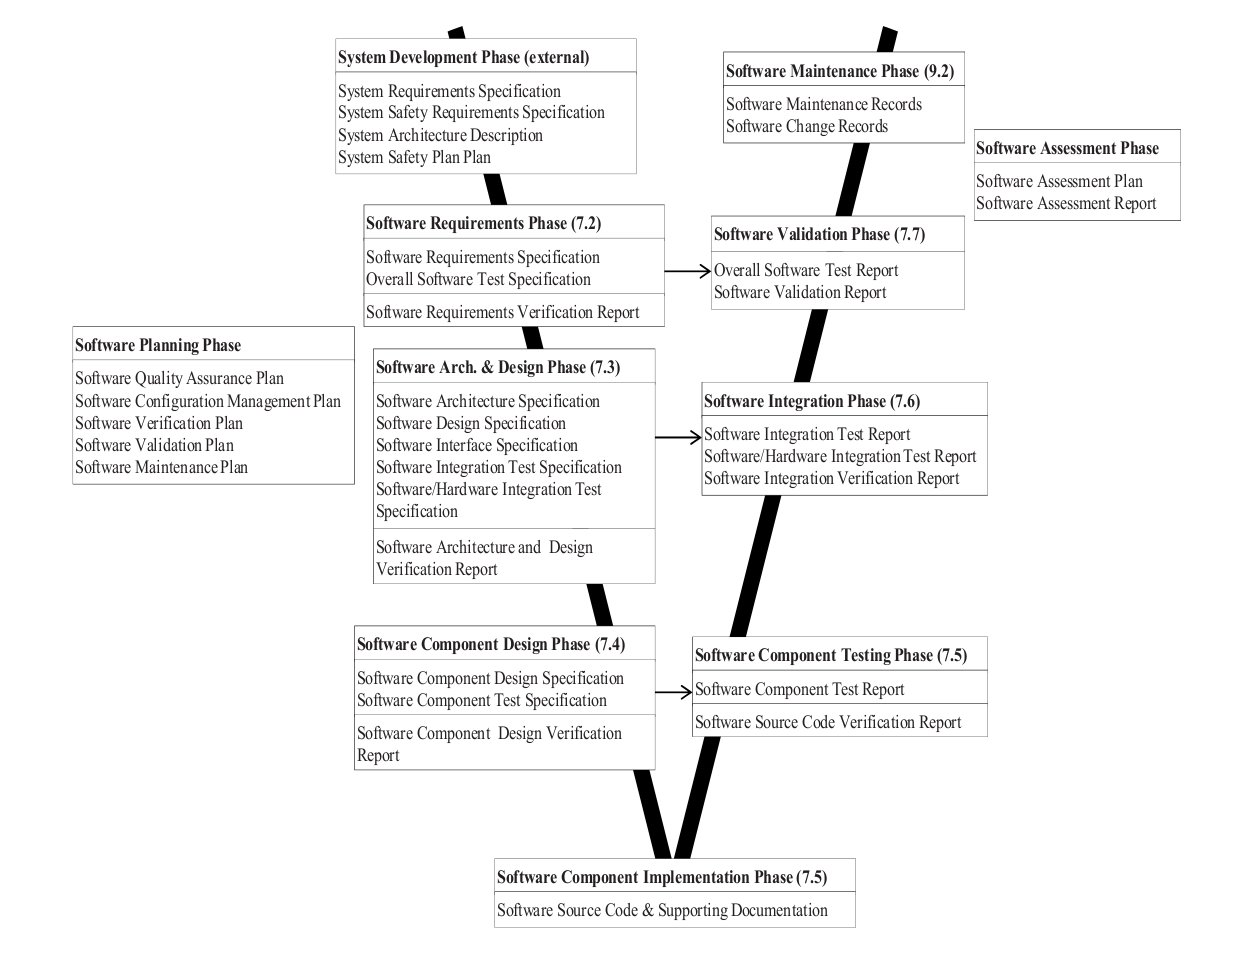
\includegraphics[width=\textwidth]{V-Model}
  \caption{General Development Lifecycle~\cite{EN-50128}}
  \label{fig:develop-lifecycle-cenelec}
\end{figure}

The recommended SW development lifecycle model in CENELEC EN 50128 is the
V-model as shown in Figure~\ref{fig:develop-lifecycle-cenelec}. It consists of
the SW planning phase in the beginning, the SW assessment phase at the end and
the following development phases:

\begin{itemize}
\item System Development Phase
\item SW Development Phases
  \begin{itemize}
  \item SW Requirements Phase
  \item SW Architecture and Design Phase
  \item SW Component Design Phase
  \item SW Component Implementation Phase
  \end{itemize}
\item SW Test / Validation Phases
  \begin{itemize}
  \item SW Validation Phase
  \item SW Integration Phase
  \item SW Component Testing Phase
  \end{itemize}
\end{itemize}

Each of the SW development phases shall have an appropriate test / validation
counterpart, as illustrated in the V form of the lifecycle. The implementation
of this generic process shall in particular focus on the usage of formal
methods. This has the following primary objectives:

\begin{itemize}
\item Increase the quality of the product wrt. safety
\item Allow for early discovery of errors in the  specifications
\item Replacement of manual steps by automatic transformations with proven
  properties
\end{itemize}

For each of the development phases of the lifecycle model of the standard, we
will propose how formal methods can be used.

\subsection{System Development Phase}
\label{sec:syst-devel-phase}

{\bf Objective:} In the system development phase, the requirements of the system
and its safety requirements shall be formalized. There shall also be a
description of the overall system architecture, preferably in a suitable
graphical modeling language\footnote{e.g. SysML~\cite{SysMLSpec}}, forming the
basis for a model-driven engineering approach. Such a model shall be refined in
the later phases, e.g., with a behavioral model. It shall serve for
documentation purposes, provide requirements traceability and parts of it will
be refined up to the algorithmic model of the executable code.

{\bf Formal Methods:} The system requirements and the safety requirements shall
be formalized in appropriate formal languages. In the system development phase,
this will be a rather high level modeling of the properties. Where possible, the
requirements will be referring the system architecture model to facilitate
traceability in later phases.

The formalization of the requirements allows for the verification of
consistency, i.e., non-contradiction of the properties. This can be done to
ensure the internal consistency of the system requirements and the safety
requirements, as well as for the consistency of the system requirements
wrt. safety requirements. Tracing of these requirements to the specification
will ensure their completeness.

Any discovered deviation from the specification shall be documented. The
documented deviation shall then be used to enhance the informal system
specification, either by removing inconsistencies from or resolving ambiguities
in the specification.

{\bf Documents:} The documents to produce in this phase are the system safety
plan, the system requirements specification, the system architecture description
and the software / hardware interface definition. The system safety plan
explains the overall approach to ensure safety in the developed system. The
system requirements specification describes all requirements of the system in a
formal language. This phase shall also produce the system architecture
specification and SW / HW interface definition which specify how the SW and the
HW interact and the location of the boundary between the two.

{\bf Detailed Description:}

{\Huge \bf TODO}

\subsection{SW Development Phase}
\label{sec:sw-development-phase}

\subsubsection{SW Requirements Phase}
\label{sec:sw-requ-phase}

{\bf Objective:} In this phase, all the SW requirements shall be formalized
based on the results of the preceding phase, i.e., the formal system
requirements, the formal safety requirements and the system architecture
specification. The part of the system model concerning the software will further
be refined, ensuring traceability of the software requirements. All existing
constraints of the constraints between HW and SW will be taken into account.

{\bf Formal Methods:} The SW requirements shall be formalized in an appropriate
formal specification language. In the software requirements phase, this will be
a rather high level modeling of the properties. If available, the requirements
shall be referenced in the part concerning SW of the refined system architecture
model.

The formalization of the SW requirements shall be used to ensure their internal
consistency and their correctness and completeness wrt. the system requirements
specification and the safety requirements specification.

The SW requirements specification shall list all functions which will be
performed by the SW, identifying each safety related function. For each
function, it will specify all required input signals and admissible values, the
expected output and the test criteria including performance and quality aspects.

A formal model of the behavior of the programmable electronic hardware shall be
established. This model shall in particular describe the modes, the transitions
between the modes and shall include the failure behavior. The correctness of
this model according to the safety specification shall be verified with
appropriate formal verification techniques. Any deviation of the behavior shall
be documented and fixed in a succeeding iteration. The documented deviations
shall be used as test cases in the SW test specification.

{\bf Documents:} The documents to produce in this phase are the SW testing
specification and the SW requirements verification report. The SW testing
specification (see 6.2, A.5) will provide the detailed approach to test the
developed SW, concertizing the approach in the SW testing plan. This shall
provide the information where formal verification will be used, in particular
where formal techniques like proofs will replace testing of the developed SW.
The SW requirements verification report will document the results of the
verification of the SW requirements specification wrt. the criteria specified in
7.2.4.22 of the standard.

{\bf Responsible:} RQM

{\bf Detailed Description:}

{\Huge\bf TODO}

\subsubsection{SW Architecture and Design Phase}
\label{sec:sw-arch-design}

{\bf Objectives:} In this phase a SW architecture shall be developed which
allows to meet the SW requirements and the necessary safety requirements. In
this phase there shall also be an evaluation of the HW / SW interaction, its
influence on the safety aspects of the system and the valuation of the usage of
already existing SW. It shall also ensure the testability and the
appropriateness for formal proofs of the resulting SW, in particular by
minimizing the complexity and the size of the safety relevant parts.

{\bf Formal Methods:} This phase shall develop a formal description of all SW
interfaces; those between different SW components and between newly developed SW
and already existing SW. This shall include pre- and postconditions, boundary
values, the behavior if those conditions are not met, memory allocation
etc. (for a full list see 7.3.4.19) ($\rightarrow$ Software interface
specification).

The architecture and design phase shall develop the description of the SW
components which will be developed. The exiting formal SW model will therefore
be refined to the SW components of the architecture. The SW requirements and
safety requirements will be refined to requirements for the components and the
necessary SIL for each components shall be identified. It shall be formally
verified, that the SW requirements for the components are consistent wrt. global
SW requirements and the safety requirements. ($\rightarrow$ Software design
specification).

For the later integration of the software, a formal behavior model of the system
into which the SW will be integrated shall be developed. To achieve this, the
behavioral model of the earlier phases shall be refined and it shall be verified
that the SW behaves as expected wrt. system into which it will be
integrated. Any deviation of this behavior shall be documented and integrated
into the software integration test specification as test-case.

{\bf Documents:} In this phase the following documents shall be produced: the
specifications for the SW architecture, the SW design and the SW interface,
there shall also be the specification for the SW integration test and for the SW
/ HW integration test. Finally the SW architecture and design verification
report will document whether this phase has been finished in accordance with
the standard.

{\bf Responsible:} DES, VER, INT

{\bf Detailed Description:}

{\Huge \bf TODO}

\subsubsection{Software Component Design Phase}
\label{sec:softw-comp-design}

{\bf Objectives:} This phase shall develop a low level specification for each of
the SW components which is correct wrt. requirements of the SW design
specification and of the SW component design specification.

{\bf Formal Methods:} This phase shall make the most elaborate use of formal
methods in the development process. The formal model describing the system shall
be further refined up to the algorithmic description on the SW component level.

Together with the specification of the various interfaces, the pre- and
postconditions, the algorithms to use and the description of the data
structures, a detailed formal model of the behavior shall be produced for each
SW component. This model shall be expressed in an appropriate formalism for
which an appropriate tool exists such that the SW and safety requirements can be
proven and the actual source code can be generated automatically.

\begin{figure}[ht]
  \centering
  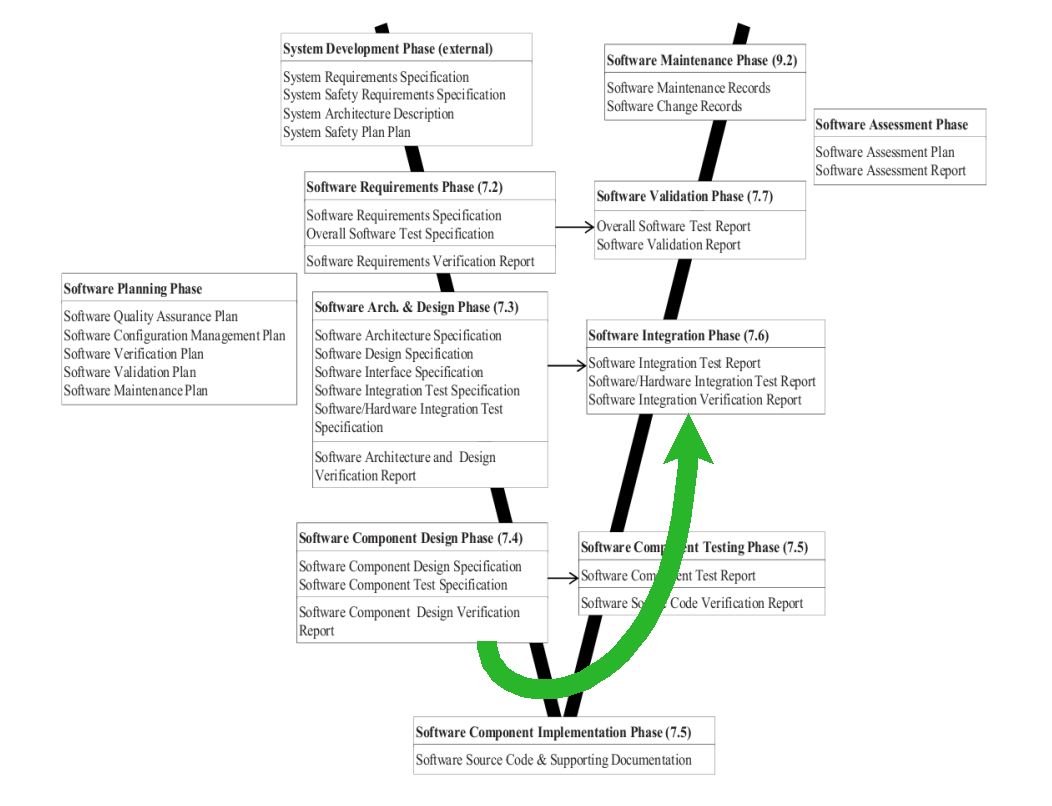
\includegraphics[width=\textwidth]{V-Model-abk}
  \caption{Formal Proof and Automatic Code Generation in V-Model}
  \label{fig:proof-code-generation}
\end{figure}

This approach will allow to replace the manual steps of component implementation
and component testing with unit-tests. The formal proofs will ensure correctness
of the generated code wrt. specification, therefore making testing
superfluous. The outline of this is shown in
Figure~\ref{fig:proof-code-generation}, where the green arrow marks the proposed
``shortcut''.

According to the standard, such an approach and the applied tools must be
appropriate according to 6.7.4.4. There will be several iterative steps until
the SW component specification will be refined enough to be eligible to
automatic code generation. A suitable formalism for this approach shall be a
formal framework which supports formal proofs of properties, supports iterative
refinement, supports refinement proofs and is suitable wrt. criteria of the
standard\footnote{e.g. the Event-B method as integrated int the Rodin
  tool~\cite{Abrial:Rodin}}.

{\bf Documents:} In this phase, the produced document will be the formal
refinement and verification report created by the formal proofs. This shall
describe the proof steps, the refinements and the necessary lemmas to prove the
properties and the refinements. The document shall also include the necessary
justifications to replace the manual step of SW component implementation and SW
component unit tests.

{\bf Responsible:} DES, VER

{\bf Detailed Description:}

{\Huge \bf TODO}

\subsubsection{Software Component Implementation Phase}
\label{sec:softw-comp-impl}

Shall be replaced by automatic code generation from formal models using
refinement techniques.

\subsubsection{Software Component Testing Phase}
\label{sec:softw-comp-test}

Shall be replaced by giving formal proofs of the generated code and showing the
adherence to all SW and safety requirements by the formal model.

\subsubsection{Software Integration Phase}
\label{sec:softw-integr-phase}

{\bf Objectives:} This phase shall demonstrate the correct functioning of the
combination of the developed SW components, in particular in their target HW
environment. The necessary tests for this phase are specified in the SW / HW
integration test specification and SW integration test specification.

{\bf Formal Methods:} Any deviation which is found in this phase shall be
documented. The results of this phase shall be used to refine the formal models
if necessary, in particular the formal models of the HW.

{\bf Documents:} The SW integration test report shall document the results from
the integration of the SW, the SW / HW integration report the results from the
integration of the developed SW on the target HW. Both shall include the test
cases, their respective results and document all details of the configuration
for the tests. The SW integration verification report shall document whether the
test reports have been written according to their respective specifications and
adhere to the relevant parts of the standard for test reports.

{\bf Responsible:} INT, VER

\subsubsection{Overall Testing / Final Validation}
\label{sec:overall-testing-}

{\bf Objectives:} The objective of this phase is to validate the adequacy of the
developed SW and its integration wrt. system requirements specification, the
functional properties and the safety related properties of the system according
to the SIL. In this phase the overall fitness for purpose of the system will be
evaluated.

{\bf Formal Methods:} This phase is executed by the VAL who will validate the
developed system. In particular, she will analyze whether the chosen combination
of techniques are appropriate wrt. standard, e.g., the use of formal proofs in
phase~\ref{sec:softw-comp-design} to replace phases~\ref{sec:softw-comp-impl}
and~\ref{sec:softw-comp-test}.

{\bf Documents:} The VAL will produce the overall SW test report in which the
VAL will document the results of additional tests she specified and executes
herself or lets TST execute them. The VAL will also produce a SW validation
report which shall document the results of the SW validation plan. The VAL will
also produce a release note which shall document any restriction of the usage of
the developed software.

{\bf Responsible:} VAL


\subsection{Conclusion}
\label{sec:conclusion-fm-process}

The focus on the application of formal methods in the proposed development
process will lead to an increased quality and reduced development cost. In
particular, formal methods will support the early detection and elimination of
design flaws through rigorous formal analysis in the in-phase iterations. Early
error detection can greatly reduce the cost, in particular for safety relevant
SW development, by avoiding to have to redo several test and validation steps.

The envisioned automatic code generation by refinement will formally proof the
correctness of the resulting SW wrt. its specification. This will increase the
quality of the resulting code, as well as eliminate the need for verification of
adherence to coding standards and for unit tests of SW components.

The proposed model-driven approach with model refinement will facilitate the
production of documentation and traceability of the requirements according to
the requirements of the standard. An important aspect to implement this approach
is the application of an appropriate supporting tool chain, in particular with
exchangeable file formats for the respective models.

A prime candidate for this is the Eclipse platform, which is well extensible and
provides support for XML based file exchange formats. It is also the basis for
model-based development tools like Topcased, provides integration for
requirements engineering tools like ProR and forms the basis for the formal
proof tool Rodin.


%%% Local Variables:
%%% mode: latex
%%% TeX-master: "wp-2.2"
%%% End:
